% Discussion of different hardware techniques
\subsubsection{FPGA-based Architectures}
\label{sec:fpga}
On Virtex-4 FPGAs, two-dimensional dynamic reconfiguration as seen in figure \ref{fig:2d} is supported. 2D Reconfiguration enables reconfiguring device portions whose height is not constrained to be the device height. This architecture of the reconfiguration core (RC) speeds up the reconfiguration time and thus the evolution time, because the individual module does not have to reconfigured column-wise (like with 1D reconfiguration). For the logic in the core candidate solutions can be used which support direct manipulation of the bitstreams. An alternative, however, is a mesh-type systolic array of parallel processing elements (PEs) from \cite{PDR}. A major feature of 2D reconfigurability is the possibility to change the functionality of the PEs by means of partial dynamically reconfiguration (PDR). This gives the system the capability to modify only small parts of the RC, while programs residing on other parts can keep on running 

One drawback of using Virtex FPGAs are the feed-through signals, mentioned in \cite{erlangen}. Each module must be implemented with all possible feed-through channels needed by other modules. Many channels reserved for a possible feed-through are redundant during run-time when the actual implementation is decided upon. Another drawback is the lack of relocation of modules accessing external pins as these are compiled for fixed locations where a direct signal line to these pins is established. 
	
% -- Plaatje 2D RC architecture ---------------------------
\begin{figure}[htb]%
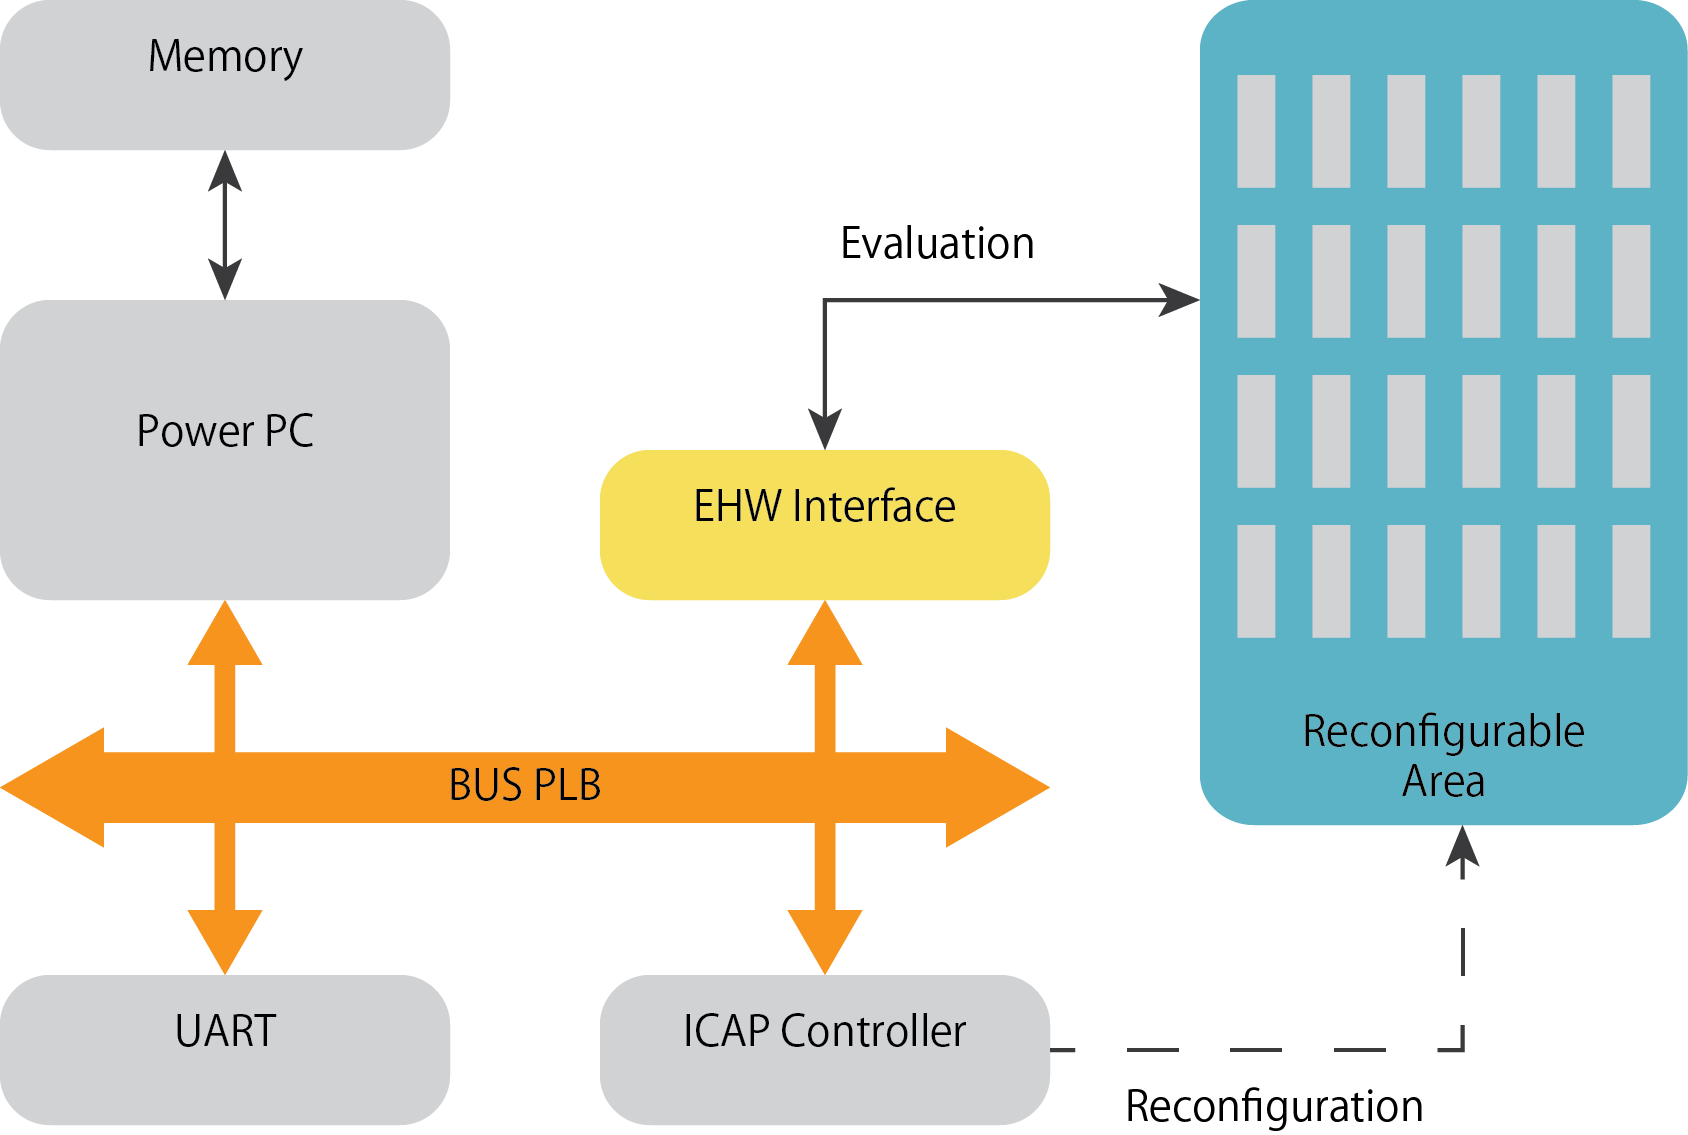
\includegraphics[width=\columnwidth]{Pictures/2D_architecture.png}%
\caption{High-level structure of a Two-Dimensional Architecture depicted in \cite{virtex4}}%
\label{fig:2d}%
\end{figure}

\subsubsection{Candidate Solutions and Direct Bitstream Manipulation}
\label{sec:candidate}
\cite{virtex4} uses direct manipulation of the bitstream in a 2D architecture for the RC to overcome the unknown and undocumented bitstream mentioned in \ref{sec:virtex4}, caused by vendor specific place and route tools. The advantages offered by this system are the overall performance (thanks to the speed-up guaranteed by the internal 2D reconfiguration) and the solutions specifiticity (thanks to a fine-grained evolution obtained through directly manipulate the cell's LUT equation). Because of 2D reconfiguration, the RC can deploy more candidate solutions, which are bidimensional arrays of cells as can be seen in figure \ref{fig:candidate}. These cells have internal flip-flops allowing the evolution of synchronous circuits.  Using these so-called candidate solutions is a common structure for \emph{evolvable hardware (EHW)} systems making use of direct bitstream manipulation \cite{virtex4}. For the cell structure of the candidate solutions the use of \emph{look-up tables (LUTs)} and a \emph{multiplexer (MUX)} is proposed. For each cell, all resources are available in one \emph{Configurable Logic Block (CLB) slice}, enabling placement of 32 cells (4 columns) in one FPGA frame. Earlier cell designs allowed only 8 cells in frame. Combined with the 2D-reconfiguration mechanism, the new architecture causes a speed up of 16x factor compared to these earlier designs. A drawback of this system is that not all FPGAs support 2D reconfiguration. Only Virtex-4 or Virtex-5 FPGAs can be used\cite{virtex4}, but this might change soon when new FPGAs are being developed support 2D reconfiguration. Another drawback is that the size of the solution space when using direct bitstream manipulation, which is rather small. By implementing mutations at different hierarchical levels the designers try to tackle this problem, but their experiments show that they still have trouble coping with complex problems requiring a high number of basic blocks.

% -- Plaatje candidates ---------------------------
\begin{figure}[htb]%
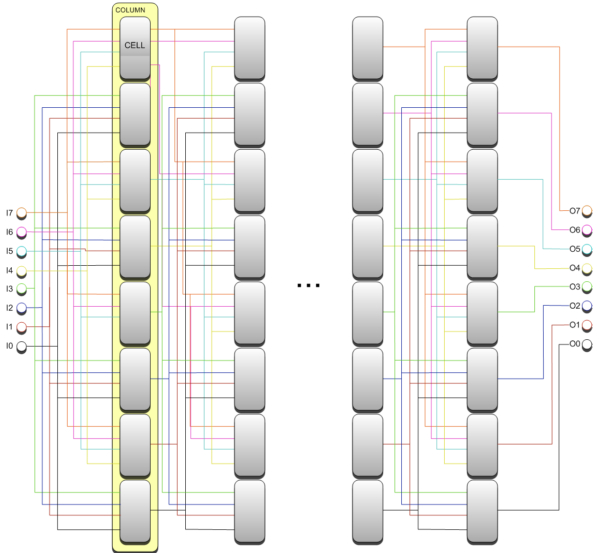
\includegraphics[width=\columnwidth]{Pictures/candidate.png}%
\caption{Internal structure of a Candidate Solution proposed in \cite{virtex4}}%
\label{fig:candidate}%
\end{figure}

\subsubsection{Systolic array of PEs and Optimized PDR}
\label{sec:PDR}
Other than \cite{virtex4}, \cite{PDR} uses a systolic array of PEs. In this approach, each PE is a basic computation unit able to perform a single operation on the data take from their close neighbors. A good thing about the PE mesh is that the outputs of the PEs (east and south side) are connected to the close neighbour's input (west and north side), such that only the lowest and right-most PE has to be read for data output. This systolic approach of communication reduces the reconfiguration time and makes the architecture scalable, which is also a nice feature. The architecture can be easily extended to any other processing purposes, since new PEs can be added to the library. In addition, PEs included in this library can be reused among applications. As can be seen in fig. \ref{fig:pe}, the size of the implemented structure is 4x4, but it is scalable. 

A drawback this type of PDR is that it requires to have relocation capability, that is, to configure the same reconfigurable module in different positions of the device, using a single bitstream as data source. FPGAs have an Internal Configuration Access Port (ICAP), which enables embedded microprocessors such as a MicroBlaze to write to FPGA configuration memory. However, HWICAP provided by Xilinx, does not support relocation. This is why the \emph{Reconfigurable Engine (RE)} is built, to place the PE as ordered by the processor in the correct position of the PE matrix. In order to implement this RE, an external DDR2 memory bank and a dedicated Native Port Interface (NPI) protocol (for connecting the RE to the memory controller) have to be added as well.

\cite{PDR} describes an implementation of this RE, which enhances the regular ICAP. Here, only the body of the bitstream (cutting of the header and the tail) is stored. Adding the header and the tail of the bitstream at runtime has two additional advantages: it allows having a unique bitstream for each PE that can be configured in any position of the array and reduces the data transference time from the external memory. 

A good thing is that the designer used the requirement of an RE also to further reduce the reconfiguration time. In addition, the FPGA is overclocked by 2,5x and internal memory is also included to avoid pasting the same configuration module in different positions of the architecture. These optimizations of the PDR recude the reconfiguration time. 


% -- Plaatje systolic PE array architecture ---------------------------
\begin{figure}[htb]%
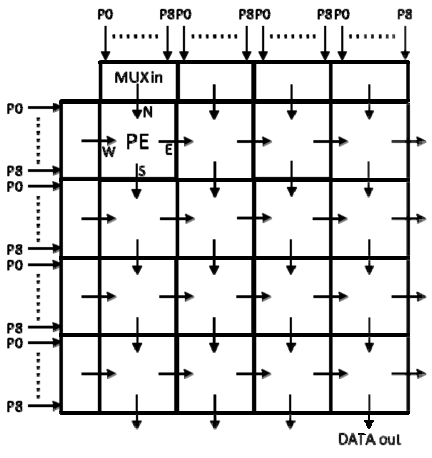
\includegraphics[width=\columnwidth]{Pictures/PE}%
\caption{Systolic array of PEs introduced by \cite{PDR}}%
\label{fig:pe}%
\end{figure}

\subsubsection{Erlangen Slot Machine}
The \emph{Erlangen Slot Machine (ESM)} presented in \cite{erlangen} deals with the three drawbacks of FPGA-based reconfigurable computers, which are: fixed pins are spread around the device causing the I/O dilemma, the inter-module dilemma and the local memory dilemma. 

First, the I/O dilemma caused by fixed pins spread around the device is solved by connecting all bottom pins from the FPGA to an interface controller realizing a crossbar, as can be seen in figure \ref{fig:erlangen}. It connects FPGA pins to peripherals automatically based on the slot position of a placed module. This I/O rerouting principle is done without reconfiguration of the crossbar FPGA.

Second, the memory dilemma has been solved. In default Virtex-II FPGAs, a module can only occupy the memory inside its physical slot boundary. Storing data in off-chip memories is therefore the only solution. In the \emph{ESM}, six SRAM banks are connected to the FPGA. Since these banks are placed at the opposite side as the crossbar, a module will connect to peripherals from one side, while the other side will be used for temporally storing computational data. In order to use a SRAM bank (called a slot), the module must have at least a width of three micro-slots, in which the total device is divided as can be seen in figure \ref{fig:erlangen}. This organization simplifies relocation, enabling a partially reconfigurable computing system and enables the availability of equal resources for each module.

Finally, the inter-module communication dilemma is dealt with. The ESM uses a combination of bus-macros, shared memory, RMB (Reconfigurable Multiple Bus) and a crossbar to take away the limiting factor for the wide use of partial dynamic reconfiguration (\cite{erlangen}).

Despite all these promises, one must not look past the bulkiness of this design. The paper first criticizes FPGAs by their feed-through signals (see \ref{sec:fpga}) and their three limitations in reconfigurable computers. Then, the proposed design contains \emph{two FPGAs}, decorated with all kinds of memory banks, crossbars and CPLDs. In order to overcome all issues accompanying FPGAs the design of \cite{erlangen} requires a lot of devices, making it a costly architecture. Also, the manufacture of the \emph{ESM} requires many steps which caused the first series to be only 15 systems. Given the complexity of the system it has little chance of becoming a product suitable for mass production.


% -- Plaatje ESM ---------------------------
\begin{figure}[htb]%
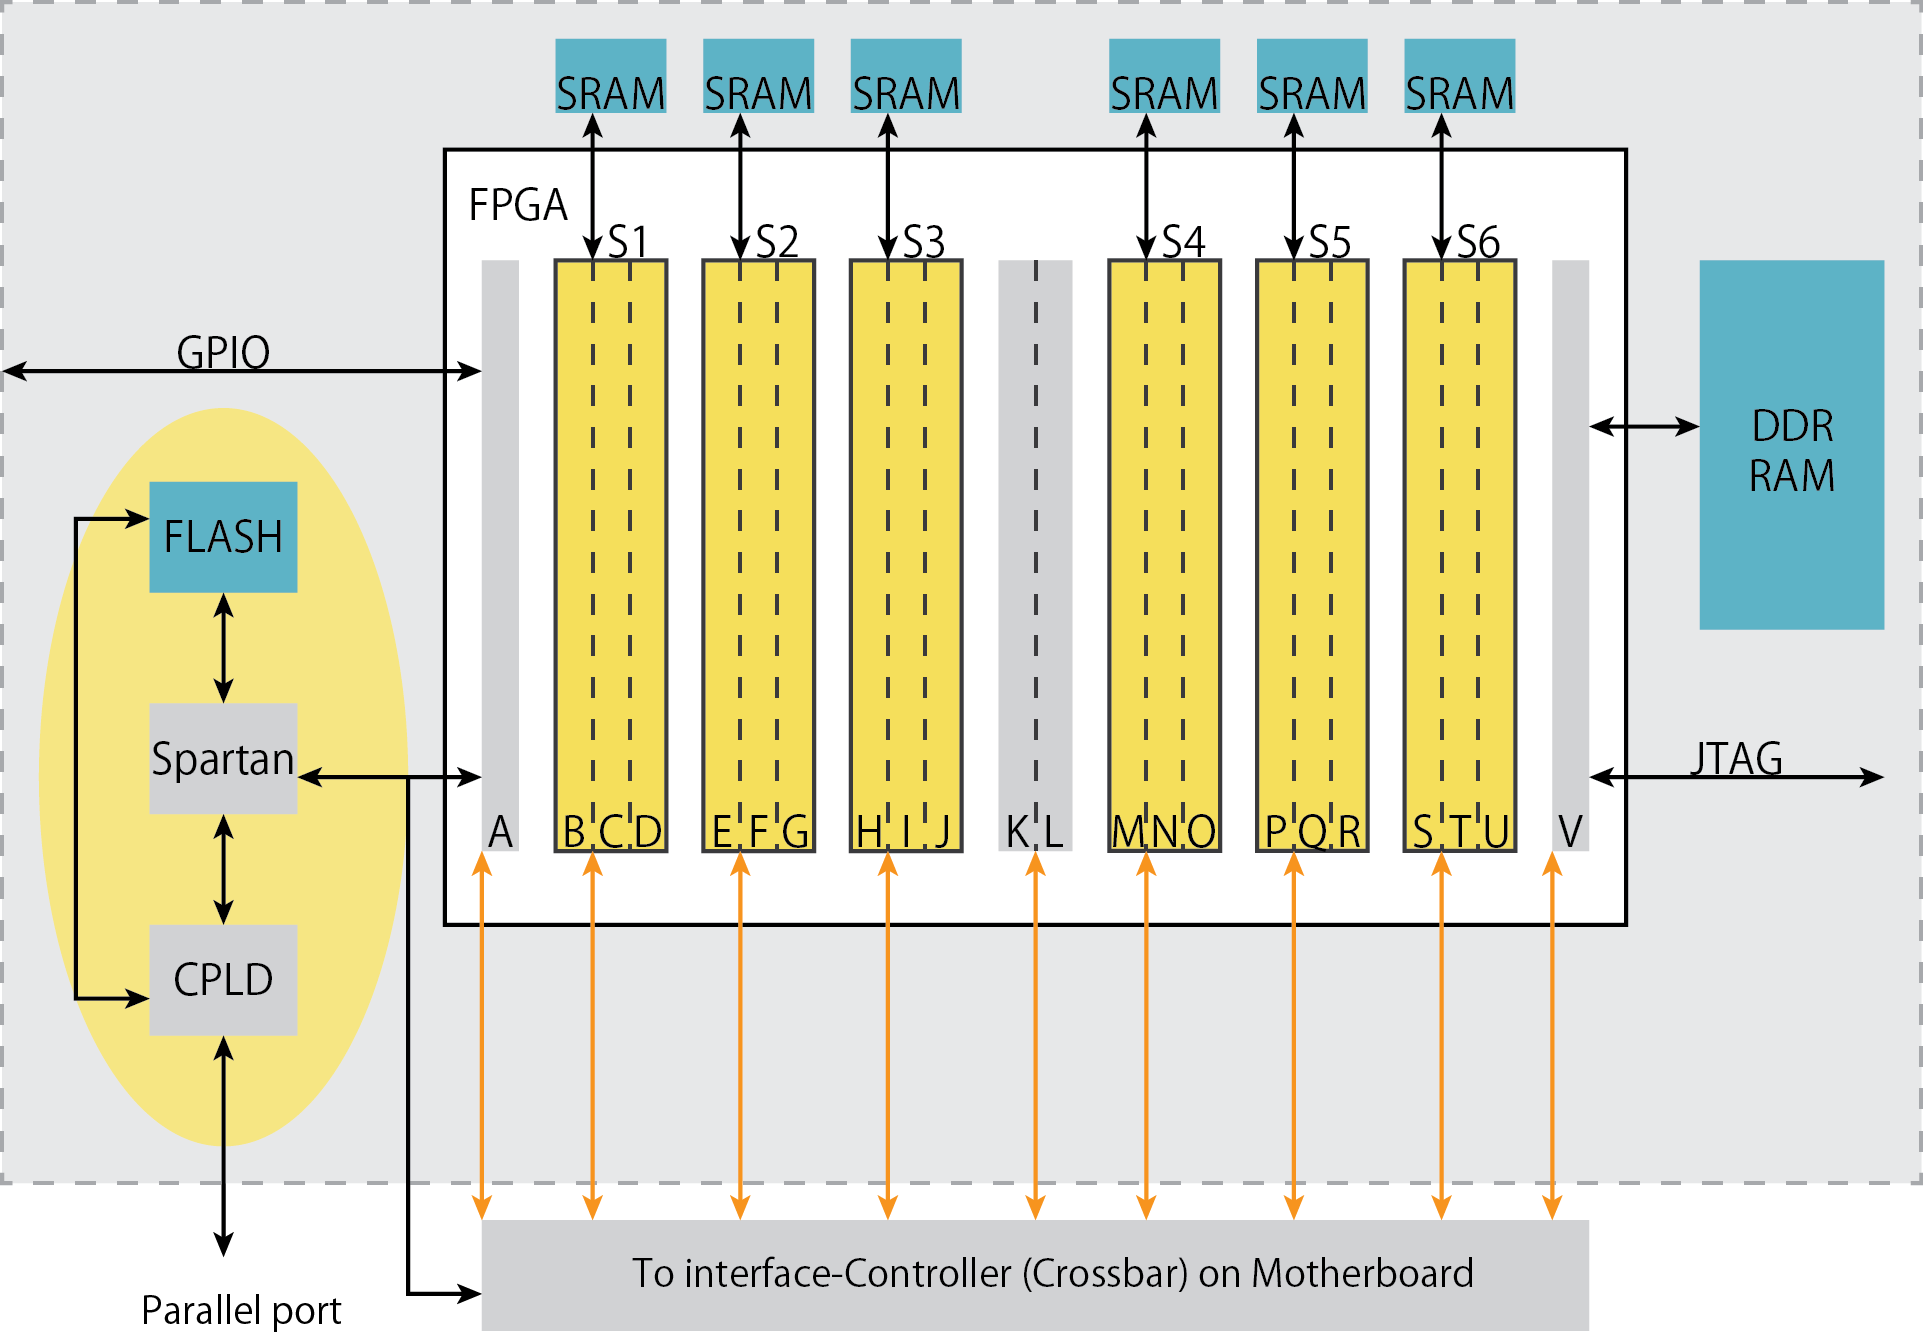
\includegraphics[width=\columnwidth]{Pictures/erlangen}%
\caption{Architecture of the ESM board. Three consecutive micro-slots define a macro-slot, which can access one full external SRAM bank.}%
\label{fig:erlangen}%
\end{figure}
